\documentclass[tikz, border=3mm]{standalone}
\usetikzlibrary{matrix}
\usepackage{amsmath}
\usetikzlibrary{shapes.arrows}
\tikzset{
	source/.pic = {
		\draw (0.5, 0.7) -- ++(0, -0.2) --
		      ++(-0.5, 0) -- ++(0, 0.5) --
		      ++(-0.7, 0) -- ++(0, -2) --
		      ++(0.7, 0) -- ++(0, 0.5) --
		      ++(0.5, 0) -- ++(0, -0.2);
	},
	detector/.pic = {
		\draw [fill=gray] (-1, 1) rectangle (1, -1);
		\draw (-0.8, 1) -- ++(0, -2);
	},
	slab/.pic = {
		\draw [fill=gray!50] (-0.2, 2) rectangle (0.2, -2);
	},
	human/.pic = {
		\draw [fill=gray] (0, 0) 
		.. controls ++(180:-1) and ++(-90: 1) .. ( 2, 1)
		.. controls ++(-90:-1) and ++(180:-1) .. ( 0, 2)
		.. controls ++(180: 1) and ++(-90:-1) .. (-2, 1)
		.. controls ++(-90: 1) and ++(180: 1) .. ( 0, 0);
		\draw [fill=white] (0, 1.5) ellipse (0.8 and 1);
		\draw (-.1, 2.49) to [in=180, out=30] ++(0.1, 0.2) to [in=150, out=0] ++(0.1, -0.2);
		\path[thick, fill=white] (-.1, 2.48) to [in=180, out=30] ++(0.1, 0.2) to [in=150, out=0] ++(0.1, -0.2) --cycle;
	}
}

\begin{document}
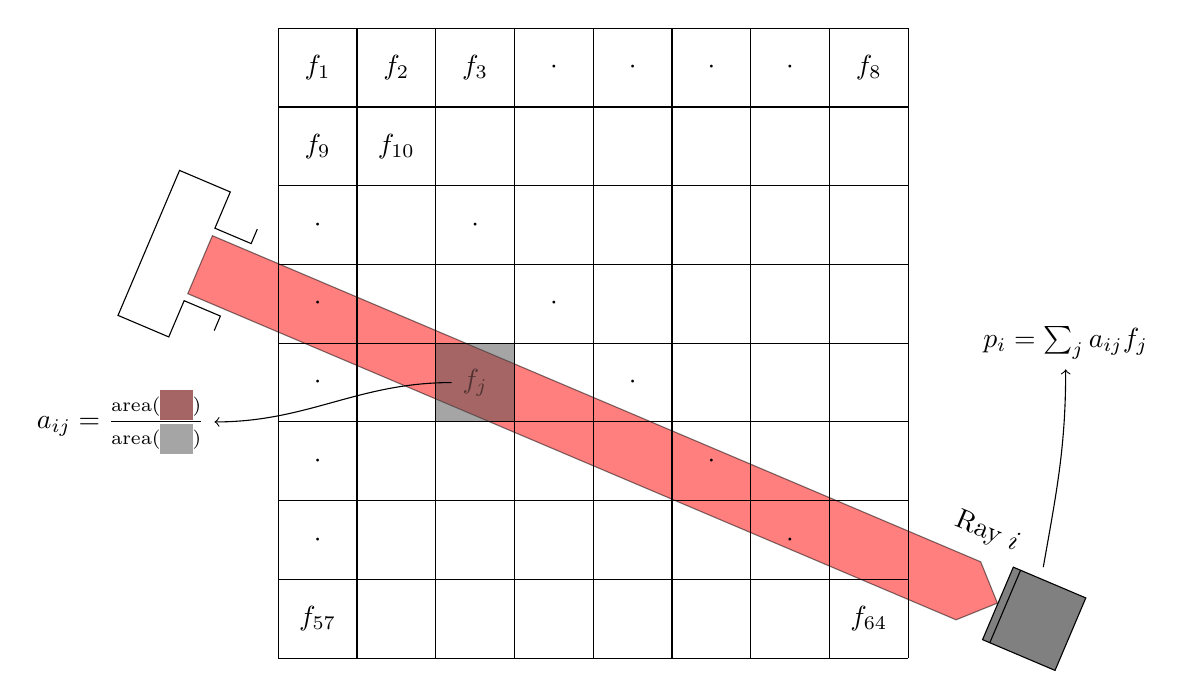
\begin{tikzpicture}
	\def\size{8}
	\node[
		draw, fill=red, single arrow, opacity=0.5,
		minimum height=11cm, minimum width=8mm,
		single arrow head extend=0mm,
		anchor=west, rotate=-23
	] at (-1, -3) {};
	\node [rotate=-23] at (9., -6.4) {Ray \( i \)};
	\node [minimum height=1cm, minimum width=1cm, fill=black!70, opacity=0.5] at (2.5, -4.5) {\( f_{j} \)};
	\node (anno) at (-2, -5) {%
			\( a_{ij} = \frac{%
				\mathrm{area}(\tikz[anchor=base, baseline]{\node [fill=red,minimum height=0.3cm, minimum width=0.3cm, opacity=0.5] {\phantom{a}}; \node [fill=black!70,minimum height=0.3cm, minimum width=0.3cm, opacity=0.5] {\phantom{a}};})
			}{%
				\mathrm{area}(\tikz[anchor=base, baseline]\node [fill=black!70,minimum height=0.3cm, minimum width=0.3cm, opacity=0.5] {\phantom{a}} ;)
			}%
		\)%
	};
	\draw [->] (2.2, -4.5) to[out=180, in=0] (anno);
	\foreach [count=\i] \x in {0,...,\size}
	{
		\draw  (\x, 0) -- ++(0, -\size);
	}
	\foreach [count=\j] \y in {0,...,-\size}
	{
		\draw (0, \y) -- ++(\size, 0);
	}
	\node at (0.5, -0.5) {\( f_1 \)};
	\node at (1.5, -0.5) {\( f_2 \)};
	\node at (2.5, -0.5) {\( f_3 \)};
	\node at (3.5, -0.5) {\( \cdot \)};
	\node at (4.5, -0.5) {\( \cdot \)};
	\node at (5.5, -0.5) {\( \cdot \)};
	\node at (6.5, -0.5) {\( \cdot \)};
	\node at (7.5, -0.5) {\( f_8 \)};
	\node at (0.5, -1.5) {\( f_9 \)};
	\node at (0.5, -2.5) {\( \cdot \)};
	\node at (0.5, -3.5) {\( \cdot \)};
	\node at (0.5, -4.5) {\( \cdot \)};
	\node at (0.5, -5.5) {\( \cdot \)};
	\node at (0.5, -6.5) {\( \cdot \)};
	\node at (1.5, -1.5) {\( f_{10} \)};
	\node at (0.5, -7.5) {\( f_{57} \)};
	\node at (7.5, -7.5) {\( f_{64} \)};
	\node at (2.5, -2.5) {\( \cdot \)};
	\node at (3.5, -3.5) {\( \cdot \)};
	\node at (4.5, -4.5) {\( \cdot \)};
	\node at (5.5, -5.5) {\( \cdot \)};
	\node at (6.5, -6.5) {\( \cdot \)};
	\pic[rotate=-23] at (-1, -3) {source};
	\pic[rotate=-23,scale=0.5, local bounding box=detector] at (9.6, -7.5) {detector};
	\node (calc) at (10, -4) {\( p_i = \sum_j a_{ij} f_j \)};
	\draw [->] (detector) to[out=80, in=-90] (calc);
\end{tikzpicture}
\end{document}
